
%(BEGIN_QUESTION)
% Copyright 2010, Tony R. Kuphaldt, released under the Creative Commons Attribution License (v 1.0)
% This means you may do almost anything with this work of mine, so long as you give me proper credit

Read and outline the ``Channel Arbitration'' subsection of the ``Digital Data Communication Theory'' section of the ``Digital Data Acquisition and Networks'' chapter in your {\it Lessons In Industrial Instrumentation} textbook.  Note the page numbers where important illustrations, photographs, equations, tables, and other relevant details are found.  Prepare to thoughtfully discuss with your instructor and classmates the concepts and examples explored in this reading.

\underbar{file i04403}
%(END_QUESTION)





%(BEGIN_ANSWER)


%(END_ANSWER)





%(BEGIN_NOTES)

Simplex = one-way communication.  Duplex = two-way communication.  Half-duplex = two-way, one way at a time.  Full-duplex = two-way simultaneous.

\vskip 10pt

Some method must be devised to limit devices from ``colliding'' on a half-duplex network.  This is called channel arbitration:

\vskip 5pt
\item{} Master-slave: only one device (the master) can initiate transmission.  All other devices (slaves) can merely reply to the master.  Network reliability utterly dependent upon the master's correct operation.  {\it e.g. HART, Modbus}
\vskip 5pt
\item{} Token-passing: only the device in possession of the token can initiate transmission (serial mastership).  Greater reliability than master-slave (no longer dependent on a single master device), but problems can arise if the network severs.  {\it e.g. Token Ring, Honeywell LCN (for the ``TDC 3000'' control system)}
\vskip 5pt
\item{} Time Division Multiple Access (TDMA): each device has a pre-schedule time slot in which to speak.  Greater reliability than token-passing and more time-efficient than master-slave, but still dependent on a master device to set the schedule and maintain synchronization.  {\it e.g. WirelessHART radio, ISA100.11a radio, GSM cell phones}
\vskip 5pt
\item{} Carrier-Sense Multiple Access (CSMA): any device can initiate transmission, following a period of silence (carrier sense).  ``Jabbering'' (when a device transmits incessantly) is able to freeze any CSMA network. 
\begin{itemize}

\item{} CSMA/BA: after collision, devices re-try in order of pre-assigned priority. {\it e.g. DeviceNet, CAN bus}
\item{} CSMA/CA: devices must wait for different pre-assigned times of silence before transmitting.  {\it WLAN}
\end{itemize}
\end{itemize}










\vskip 20pt \vbox{\hrule \hbox{\strut \vrule{} {\bf Suggestions for Socratic discussion} \vrule} \hrule}

\begin{itemize}
\item{} Identify and describe the channel arbitration method used by HART instrument networks.
\item{} Identify and describe the channel arbitration method used by Modbus networks.
\item{} Identify and describe the channel arbitration method used by Honeywell LCN networks.
\item{} Identify and describe the channel arbitration method used by wired Ethernet networks.
\item{} Identify and describe the channel arbitration method used by DeviceNet and CANbus networks.
\item{} Identify and describe the channel arbitration method used by WLAN wireless networks.
\item{} Identify and describe the channel arbitration method used by GSM cell phone networks.
\item{} Identify ways in which a {\it master-slave} communications network can fail.
\item{} Identify ways in which a {\it token-passing} communications network can fail.
\item{} Identify ways in which a {\it CSMA} communications network can fail.
\item{} Identify ways in which a {\it TDMA} communications network can fail.
\end{itemize}




\vfil \eject

$$\includegraphics[width=15.5cm]{i04403x01.eps}$$

\vskip 20pt \vbox{\hrule \hbox{\strut \vrule{} {\bf Suggestions for Socratic discussion} \vrule} \hrule}

\begin{itemize}
\item{} Describe communication between two or more of the nodes on this network, using master/slave arbitration.
\item{} Describe communication between two or more of the nodes on this network, using token-passing arbitration.
\item{} Describe communication between two or more of the nodes on this network, using CSMA/CD arbitration.
\item{} Describe communication between two or more of the nodes on this network, using CSMA/BA arbitration.
\item{} Describe communication between two or more of the nodes on this network, using CSMA/CA arbitration.
\end{itemize}








\vfil \eject

\noindent
{\bf Prep Quiz:}

A {\it CSMA/CD} (CSMA-``collision detection'')  arbitration strategy is one where:

\begin{itemize}
\item{} Devices may transmit at any time, but must wait some random time after a collision occurs
\vskip 5pt 
\item{} Devices may transmit at any time, but must wait in ranked order after a collision occurs
\vskip 5pt 
\item{} Devices may transmit only after some pre-determined amount of network silent time
\vskip 5pt 
\item{} Only one device is allowed to initiate communication; all other devices may only reply
\vskip 5pt 
\item{} Each device on the network has a pre-determined ``time slot'' in which to transmit
\vskip 5pt 
\item{} Pyro the magic elf arbitrarily decides when devices may transmit, in his infinite wisdom
\end{itemize}








\vfil \eject

\noindent
{\bf Prep Quiz:}

A {\it CSMA/BA} (CSMA-``bitwise arbitration'') strategy is one where:

\begin{itemize}
\item{} Devices may transmit at any time, but must wait some random time after a collision occurs
\vskip 5pt 
\item{} Devices may transmit at any time, but must wait in ranked order after a collision occurs
\vskip 5pt 
\item{} Devices may transmit only after some pre-determined amount of network silent time
\vskip 5pt 
\item{} Only one device is allowed to initiate communication; all other devices may only reply
\vskip 5pt 
\item{} Each device on the network has a pre-determined ``time slot'' in which to transmit
\vskip 5pt 
\item{} Pyro the magic elf arbitrarily decides when devices may transmit, in his infinite wisdom
\end{itemize}








\vfil \eject

\noindent
{\bf Prep Quiz:}

A {\it CSMA/CA} (CSMA-``collision avoidance'') arbitration strategy is one where:

\begin{itemize}
\item{} Devices may transmit at any time, but must wait some random time after a collision occurs
\vskip 5pt 
\item{} Devices may transmit at any time, but must wait in ranked order after a collision occurs
\vskip 5pt 
\item{} Devices may transmit only after some pre-determined amount of network silent time
\vskip 5pt 
\item{} Only one device is allowed to initiate communication; all other devices may only reply
\vskip 5pt 
\item{} Each device on the network has a pre-determined ``time slot'' in which to transmit
\vskip 5pt 
\item{} Pyro the magic elf arbitrarily decides when devices may transmit, in his infinite wisdom
\end{itemize}











\vfil \eject

\noindent
{\bf Prep Quiz:}

A {\it TDMA} arbitration strategy is one where:

\begin{itemize}
\item{} Devices may transmit at any time, but must wait some random time after a collision occurs
\vskip 5pt 
\item{} Devices may transmit at any time, but must wait in ranked order after a collision occurs
\vskip 5pt 
\item{} Devices may transmit only after some pre-determined amount of network silent time
\vskip 5pt 
\item{} Only one device is allowed to initiate communication; all other devices may only reply
\vskip 5pt 
\item{} Each device on the network has a pre-determined ``time slot'' in which to transmit
\vskip 5pt 
\item{} Pyro the magic elf arbitrarily decides when devices may transmit, in his infinite wisdom
\end{itemize}

%INDEX% Reading assignment: Lessons In Industrial Instrumentation, Digital data and networks (channel arbitration)

%(END_NOTES)

